\chapter{Analysis and methodology}

\section{Time series forecasting - general model structure}
A model for time series forecasting must be structured in the following way.
As input, it must take a sequence of vectors, with each vector representing a single point in time, and each element of the vector representing an element of the time series.
As output, it must similarly produce a sequence of multivariate vectors.
In the case that the model is forecasting only a single time series, the output vectors will have only a single element each.
This structure is presented in Figure \ref{fig:forecast-model}.

\begin{figure}
	\centering
	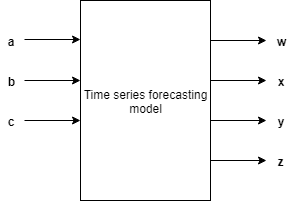
\includegraphics[width=0.35\linewidth]{images/forecast-model}
	\caption{A time series forecasting model takes a sequence of vectors, $\va, \vb, \vc$, as input and produces a sequence of vectors, $\vw, \vx, \vy, \vz$, as output. Note the number of input and output vectors is able to vary.}
	\label{fig:forecast-model}
\end{figure}

This structure is identical to that used for neural machine translation (NMT), where a source sentence/phrase is translated from one language, say English, to another language such as Dutch \citep{Cho2014}.
In NMT, a word is represented by a vector, and a sentence is represented by a sequence of vectors.

\par
This section will investigate the performance of several of the best performing NMT architectures when applied to time series forecasting.

\subsection{Investigated models}
The following NMT models will be investigated and their results in time series forecasting compared
\begin{itemize}
	\item sequence to sequence (S2S) \citep{Cho2014a} long short term memory (LSTM) \citep{hochreiter1997long}
	\item S2S LSTM with attention \citep{luong2015effective}
	\item S2S gated recurrent unit (GRU) \citep{Cho2014a}
	\item S2S GRU with attention
	\item Transformer \citep{Vaswani2017}
\end{itemize}

Additionally, I will compare them to the following traditional methods
\begin{itemize}
	\item ARIMA and related methods
	\item support vector regression
	\item I'll probably add a few more as I further work on the state of the art section.
\end{itemize}

\subsection{Evaluation tasks}
The following time series forecasting tasks will be used to evaluate the models
\begin{itemize}
	\item forecasting a pure sine wave given its past values
	\item forecasting a sine wave with normally distributed noise given its past values
	\item forecasting a signal comprised of several sine waves with normally distributed noise given past values
	\item forecasting the Bruny Island load data - no priority given to special days.
\end{itemize}

\subsection{Evaluation Results}

\section{Transformer}
\hl{My preliminary investigations show that the transformer architecture is the best, or at least equal best but likely with less expensive training. This is consistent with \protect\cite{Song2017} and \protect\cite{Vaswani2017}}\\
\par
The transformer is a neural network architecture that is currently the state of the art in NMT \citep{Vaswani2017}.
This architecture will be discussed in detail. 

\subsection{Overview}
overview of the transformer architecture.
\begin{itemize}
	\item encoder and decoder
	\item input embedding
	\item positional encoding
	\item multi-head attention
	\item residual connections
	\item feed forward
	\item layer normalization
	\item 
\end{itemize}

\subsection{Input embedding}
convolutional embedding as per \citep{Song2017} (a paper using the transformer architecture to perform classification based on time series).

\subsection{Positional encoding}
Every input vector, $\vb_i$, has a vector added to it, $\vp_i$, depending on its position, $i$, in the input.
$\vp_i$ is trainable - it is drawn from $\vtheta$.

\subsection{multi-head attention}
I need to research this further before writing about it.

\subsection{residual connections}

\subsection{Feedforward}

\subsection{Normalization}

\subsection{etc.}

\subsection{Training}
Discuss how the decoder is used in training and inference modes.
Causality, iterative inference.
	